\documentclass{article}
\usepackage[swedish]{babel}
\usepackage[utf8]{inputenc}
\usepackage[T1]{fontenc}

%Lägger till Referenser i Innehållsförteckningen
\usepackage{tocbibind}
\usepackage{float}
\usepackage{amsmath}
\usepackage{parskip}
\usepackage{todonotes}
\usepackage{url}
\usepackage{hyperref}
\usepackage{multicol}

\title{Utveckling av modulärt larmsystem baserat på MD407-enkortsdatorer}

\author{\large Grupp 13\\Filip Borg, Gustav Fåhraeus, Josef Karlsson,\\
Erik Nilsson, Adam Thörnblom, Ben Wooldridge}
\date{Läsperiod 1, HT-2019\\DAT290 Datatekniskt projekt\\Datateknik}

% I utvärderingen granskas hur väl studenterna i sina rapporter har lyckats visa att de genom de teknikutvärderingar, konstruktionsval, tester och analys som de har gjort har förstått de problem de har ställts inför, samt hur de på basis av denna förståelse och utifrån rådande förutsättningar har lyckats agera för att lösa dessa problem.

% Kriterierna är läsarorienterade vilket innebär att de ska bedöma en utomstående läsaresmöjligheter att förstå rapporten. Rapporten ska först och främst ses som ett dokument vars läsare finns inom organisationen där arbetet sker,men det ska kunna läsas och förstås av personer som inte har jobbat med och därför inte är insatta i projektet, exempelvis en nyanställd som inte känner till projektet och dess bakgrund, en anställd i en annan organisation med liknande verksamhet eller en ingenjörsstudent inom datateknik som har gått en liknande utbildning på en annanhögskola.

% En bakåtsyftande projektrapport: “Rapporten beskriver utvecklingen av…”




\begin{document}

%Titelsida
\maketitle
\pagenumbering{gobble}
\newpage

\tableofcontents
\newpage

\pagenumbering{arabic}

\section*{Beteckningar}
\begin{itemize}
    \item \textbf{MD407} – En ARM-baserad
    laborationsdator för utbildning
    \item \textbf{ARM} - En processor-arkitektur
    \item \textbf{CAN} - Controller Area Network
    \item \textbf{GPIO} - General-purpose input/output
    \item \textbf{USART} - Universal asynchronous receiver-transmitter
    \item \textbf{LED} - Light-emitting diode
    \item \textbf{AUX} - Auxiliary
\end{itemize}
\newpage

\section{Inledning}
I en undersökning\cite{brott-foretagarna} utförd av Sveriges största företagsorganisaton, \textit{Företagarna}, anger var tredje företag (n=983) att de blivit utsatta för minst ett brott någon gång under de senaste fem åren. Pontus Lindström, ansvarig för brott- och trygghetsfrågor hos Företagarna säger:
\begin{quote}
\textit{- Undersökningen bekräftar den bild vi har. Många företagare vittnar om en ökad utsatthet och om att otryggheten ökat.}
\end{quote}

25\% av de företag som blivit utsatta för minst ett brott anger att de inte anmält brottet till polisen. 36\% anger att de anmält något av brotten de utsatts för. Att anmälningsgraden är så låg tyder på att att företagen inte anser att det är värt besväret att anmäla brott till polisen. Företagen i undersökningen anger också att de känner sig tvungna att satsa stora summor på larmsystem, vilket för många enskilda firmor och handelsbolag inte alltid är genomförbart av finansiella skäl.

Baserat på denna undersökningen verkar det finnas ett behov för ett skalbart larmsystem där användaren kan justera omfattingen för larmet baserat på rådande nödvändighet och finansiell kapabilitet.

Rapporten beskriver utvecklingen av ett modulärt larmsystem som i grunden består av MD407-enkortsdatorer\cite{MD407}.

\subsection{Syfte} % Svarar på frågan "Varför"?
Projekets syfte är att utveckla ett larmsystemets som ska vara ett finansiellt dynamiskt alternativ för företag
och organisationer som har behov av skalningsbar och anpassad larmning beroende på nuvarande nödvändighet och finansiell \\ kapabilitet.
Detta uppnås genom att erbjuda mindre delsystem som kan kopplas ihop till ett större centraliserat system.

Systemet ökar översikten och säkerheten av användarens lokaler genom att implementera konfigurerbar larmning av dörrar, samt rörelse- och vibrationsdetektering.

\subsection{Mål} % Svarar på frågan "Vad"?
% I detta avsnitt beskrivs koncist samtliga övergripande tekniska mål med projektet, det vill säga, vad som ska konstrueras. De mål som anges här kommer att styra projektets utveckling. När projektet närmar sig sitt slut och den slutliga projektrapporten lämnas in kommer beställaren att kritiskt analysera hur väl projektet lyckats genom att jämföra planens mål med den tekniska konstruktion som redovisas i projektrapporten.
Ett komplett larmsystem i minimal form består av tre enheter: en dörrenhet, en rörelseenhet, och en centralenhet.
Samtliga enheter kräver varsin MD407-enkortsdator för individuell drift. För att koppla samman
fristående enheter till ett centraliserat system används en CAN-buss.
CAN-kommunikationen bygger på ett fåtal meddelanden som sköter den informationsdelning som systemet kräver. Informationen som skickas på CAN-nätverket skyddas från återuppspelningsattack där tidigare inspelad trafik återuppspelas vid ett senare tillfälle.

Dörrenheten hanterar detektering och larmning av dörrar. Vid systemuppstart kontrollerar
dörrenheten antalet dörrar kopplade på enkortsdatorn. Datarepresentationer av dessa dörrar skapas, vilket möjliggör för dörrarna att efter en förutbestämd tid utlösa lokala larm genom att en LED-lampa på den larmande dörren tänds.
Dörrarna kan skicka centrala larm via en CAN-buss till centralenheten. Tider innan respektive larm utlöses kan konfigureras från centralenheten.
Från centralenheten kan dörrar också avlarmas, vilket hindrar samtliga larm på dörren från att utlösas.

Röreleseenheten består av en rörelse- och en vibrationssensor. Om endera sensor
utlöses skickas ett centralt larm via en CAN-buss till centralenheten. Känsligheten
på rörelsesensorn konfigueras från centralenheten. Vibrationssensorn konfigueras direkt på hårdvaran.

Centralenheten hanterar konfiguration av periferienheterna, samt fungerar som en
central för samtliga larm som utlöses i systemet. Om ett centralt larm utlöses så
kan det endast ackkrediteras och nollställas via centralenheten.
\subsection{Arbetsmetod} % svarar på frågan "hur har vi gått tillväga i det tekniska utvecklingsarbetet"?

I det här avsnittet beskrivs hur den tekniska utvecklingen gått till.


\subsubsection{Utveckling}

Utvecklingen av mjukvaran har främst skett på enhetsnivå, dvs att mjukvaran på de olika enheterna utvecklats separat från varandra.
När samtlliga enheter hade uppnåt majoriteten av sin tänkta funktionalitet så bytte utvecklingen fokus till att handla om att få enheterna att kommunicera med varandra via en CAN-buss.

Periferienhets-grupperna byggde först system för att hantera initiering av relevanta GPIO portar samt debugfunktioner, och fortsatte med att implementera funktioner för avmätning av sensorerna. Funktionalitet byggdes på och det sista som utvecklades var kommunkiationen mellan periferienheterna och centralenheten.

På centralenheten utvecklades först USART, samt ett antal debugfunktioner som kunde användas av alla enheter. Implemteringen av CAN-kommunikation på centralenheten styrde mycket av hur CAN implementerades på de andra enheterna, då centralenheten är den som tar emot och skickar flest meddelanden.

Stora majoriten av mjukvaroutvecklingen och test har utförts på hårdvaran som beskrivs i rapporten, men en del av utvecklingen har skett med hjälp av simulerad hårdvara.

\subsubsection{Programbibliotek}
\label{stm}
Ett STM32F4-biblioteket har används för att bespara arbetstid.
Programbiblioteket STM32F4\cite{stm} används för:
\begin{itemize}
    \item Initieringar och avläsning av enkortsdatorernas GPIO portar.
    \item Implementation av en System Timer (SysTick).
    \item "Väntetid'-funktionalitet. (Delay-funktioner)
    \item Implementation av CAN-kommunikation.
\end{itemize}



\subsubsection{Verifikation}
\label{verifikation}
För att utvärdera huruvida larmsystemet uppnår de mål och krav som formulerats i målet används tester.
De tre undergrupperna har skrivit tester för sina respektive delsystem som försäkrar att
delsystemen fungerar enligt specifikationen. Ett test som är skrivet av en undergrupp utförs
av en annan undergrupp för att minimera partiskhet i utförandet.

Testet för det kompletta centraliserade systemet formulerades och utfördes av gruppen som helhet.

För att se samtliga testspecifikationer, samt resultat och analys, se bilaga \ref{bilaga:tester}.

\subsubsection{Fildelning och versionshantering}
Arbetsgruppen valde att använda versionshanteringstjänsten GIT för att förenkla den parallella programmeringen, och för att samla alla filer på ett ställe. GIT-filsamlingen förvarades med hjälp av tjänsten github. GIT-Tjänsten har fungerat väl och även underlättat dokumentering, då även den förvarades i filsamlingen.

\newpage
\section{Teknisk beskrivning} % Vad är utgångspunkten för i förkonstruktionsarbetet?
I det här avsnittet presenteras teknisk information som är nödvändig för att få en djupare insikt i hur den tekniska utvecklingen gått till, samt hur de olika delsystem fungerar och interagerar för att bygga upp systemet som helhet.
\subsection{Teknisk bakgrund}
Mjukvaran till larmsystemet körs på ett flertal MD407-enkortsdatorer, en för varje enhet.

\textbf{STM32-Programbibliotek}\cite{stm} är ett programbibliotek som har generellt skrivna funktioner som
redan skrivits för ARM.
\todo[inline]{Mitt förslag är att ist skriva\\
är ett programbibliotek som har vanliga funktioner som ofta används för ARM}

\textbf{Polling} är ett protokoll som frågar alla I/O Enheter kontinuerligt ifall de behöver proccesering.\subsection{Systemöversikt}

Systemet utgår från en centralenhet, kopplad till ett antal dörrenheter och rörelsenheter över en gemensam CAN-buss. Periferienheterna hanterar avmätning av sina respektive sensorer, samt begär larm via CAN-bussen vid behov. När det går ett centralt larm fortsätter larmet tills en användare slår av larmet via kommandon till centralenheten.

Dörrenheten är kopplad till ett antal strömbrytare/dörrsensorer, och larmar då en dörr är öppen för länge, först lokalt och sedan centralt.

Rörelseenheten har ett antal rörelse- och vibrationsensorer inkopplade. Rörelsesensorerna har centralt samt ett lokalt larm med det dubbla avståndet
som larmar centralt respektive lokalt när sensorn detekterar något innaför dess larmavstånd.
Rörelseenheten larmar även centralt när en vibrationssensor mäter en vibration.

En översikt av hårdvaran och hur den är kopplad finns i Figur \ref{fig:hårdvara}. Värt att notera i figuren är att den endast visar en enhet av varje typ, samt bara en sensor av varje typ, medan det i själva verket kan kopplas in ett flertal till systemet.
\begin{figure}[H] % Samma figur som projektplanen, då hårdvaran fortfarande ser likadan ut, det är värt att göra en ny innan slutgiltiga rapporten.
    \centering
    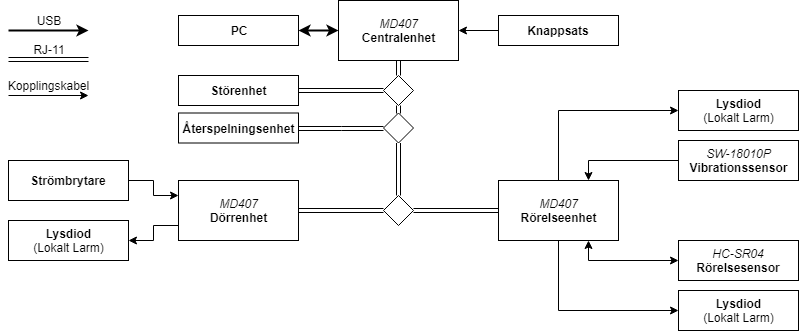
\includegraphics[width=1\textwidth]{figurer/HardvaraOversikt.png}
    \caption{Översikt över hårdvara}
    \label{fig:hårdvara}
\end{figure}

När centralenheten samt periferienheterna startar befinner de sig i konfigurationsläge, där varje enhet konfigurerar sig på lokal nivå (USART CAN-bussen, GPIO), varpå centralenheten skickar konfigurationer till periferienheterna, som de använder för att konfigurera sina respektive sensorer.
Efter att ha konfigurerats går enheterna in i var sin kontinuerlig loop. Periferienheterna mäter ständigt av sensorerna och skickar larm-meddelanden över CAN-bussen till centralenheten vid behov. Centralenheten skickar periodiskt konfigurationer till periferienheterna och larmar ifall dessa inte bekräftas.

En överblick av mjukvarans tidsflöde finns i figur \ref{fig:tidsflöde}.

\begin{figure}[H]
    \centering
    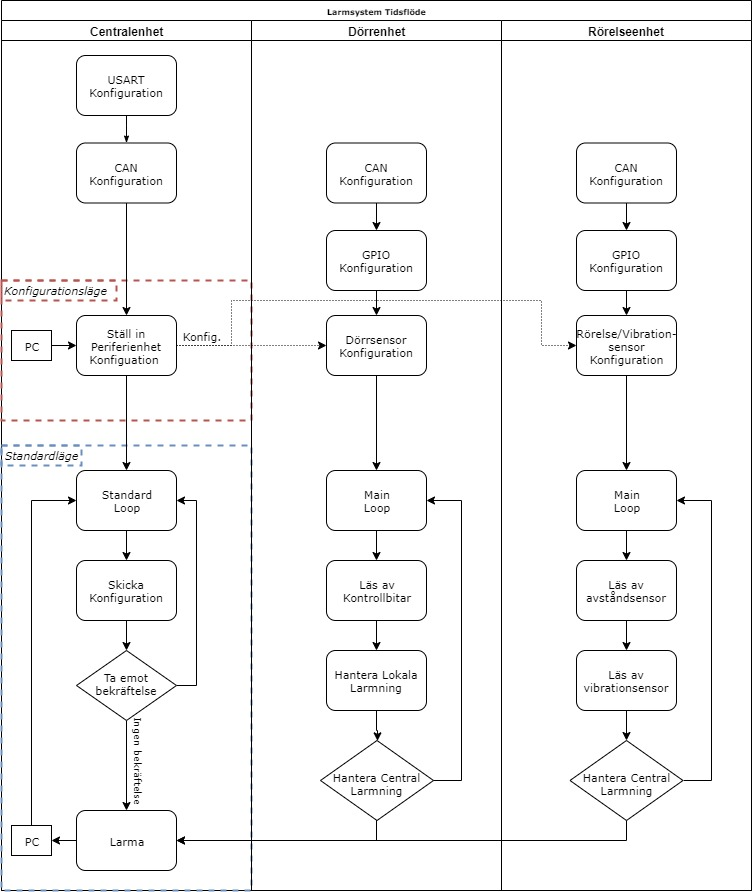
\includegraphics[width=1\textwidth]{figurer/TidsFlode.jpg}
    \caption{En översiktlig beskrivning av logik-flödet för systemets mjukvara. Övre halvan för varje enhet är en initieringsfas,
    och nedre halvan representerar enheternas 'huvudloop' som är aktiv när systemet är i drift.}
    \label{fig:tidsflöde}
\end{figure}

\subsection{CAN-kommunikation}
\label{can}
Här presenteras protokollet som har utvecklats för informationsutbyte mellan enheterna därefter förljer en implementationsbeskrivning.

\subsubsection{Beskrivning av CAN-protokollet}
Protokollet som har utvecklats för kommunikationen mellan enheterna bygger på protokollet Controller Area Network (CAN).
CAN är ett bussprotokoll som främst används för kommunikation mellan datorer och givare på fordon där det ställs höga krav på tillförlitlighet.
För att undvika kollisioner och därmed öka tillförlitligheten har CAN en dominant logisk nivå (0) som dessutom ger automatisk prioritering av meddelanden då den dominanta nivån har företräde på bussen.
Denna prioritering har använts för att ge brådskande meddelanden företräde över meddelanden som inte kräver kort responstid. I tabell \ref{tab:meddelandetyper} är de meddelandetyper som används kortfattat beskrivna. För en mer detaljerad beskrivning av protokollet och dess meddelandetyper, se bilaga \ref{bilaga:protokoll}. För att motverka en återuppspelningsattack beskriver en del av meddelandet vilken session som meddelandet tillhör. Om det sedan skickas ett meddelande för en annan session så ignoreras det.



\begin{table}[H]
	\centering
    \begin{tabular}{|l|p{0.7\textwidth}|}

		\hline
		Meddelandetyp & Används till \\ \hline \hline
		Bekräftelse		& Bekräftelse för det senast mottagna meddelandet. \\ \hline
		Skicka larm		& Talar om för centralenheten om någon dörr eller sensor larmar. \\ \hline
		Konfiguration		& Används för att skicka sensorkonfiguration och kalibrering. \\ \hline
		Tilldelning av id		& Används då centralenheten tilldelar en periferienhet dess id. \\ \hline
		Id-begäran		& Används för att begära ett id. \\ \hline

	\end{tabular}
	\caption{Meddelandetyper som används för datakommunikationen.}
	\label{tab:meddelandetyper}
\end{table}


\subsubsection{Implementation}
För hantering av CAN-meddelanden har STM-biblioteket (se \ref{stm}) använts för inledande initiering,
hantering av avbrott och att skicka meddelanden.
Utöver det har ett system utvecklats för att hantera mottagna meddelanden med hjälp av avbrott.
Hanteringsfunktionen paras ihop med filtret för tillhörande meddelande.
Hanteringsfunktionen anropas sedan av avbrottsrutinen då ett meddelande passerat filtret.
Denna lösning har valts då de flesta meddelanden naturligt hanteras med en kort hanteringsfunktion
som inte kräver input från användaren.


\subsection{USART}
För att ge användaren möjlighet att interagera med systemet har Universal asynchronous receiver-transmitter (USART) implementerats. USART sköter kommunikationen mellan mikrodatorn och den terminal som används då mikrodatorn är ansluten till en dator. Via terminalen får användaren utskrifter från programmet och har även möjlighet att ge kommandon till systemet.


\subsection{Störenhet}
För att ge möjlighet att testa systemet på ett tungt trafikerat CAN-nätverk har en störenhet utvecklats. Störenheten skickar frekvent meddelanden med slumpartat innehåll. Hastigheten är reglerbar via USART. Utöver att generera brus kan enheten också fungera som en lyssnare med avaktiverad störfunktion.

\subsection{Återspelningsenhet}
För att säkerställa att åtgärden för att hindra återspelningsattacker fungerar som den ska har en återspelningsenhet tagits fram. Enheten kopplas upp på bussen och kan därefter spela in den trafik som skickas. Inspelningsbuffern har möjlighet att lagra 1000 meddelanden som på begäran kan skickad på nytt när en attack vill simuleras. Enheten kan sköta inspelning och uppspelning samtidigt och har dessutom inställningsmöjlighet för att återupprepa uppspelningen då man spelat upp alla meddelanden.


\subsection{Delsystem }
Varje egen enhet ses som en del utav det hela systemet. Dessa tre delsystem är
centralenheten, dörrenheten och rörelseenheten. I det här avsnittet beskrivs de
olika delsystemen.
\subsubsection{Centralenheten}
\label{subsec:centralenhet}

Centralenheten styr och har uppsikt över periferienheterna enligt figur \ref{fig:centralflöde}.
Inställningar görs via USART med kommandon enligt bilaga \ref{kommandon}, varpå de vidarebefordras till rätt periferienhet via CAN.

\begin{figure}[H]
    \centering
    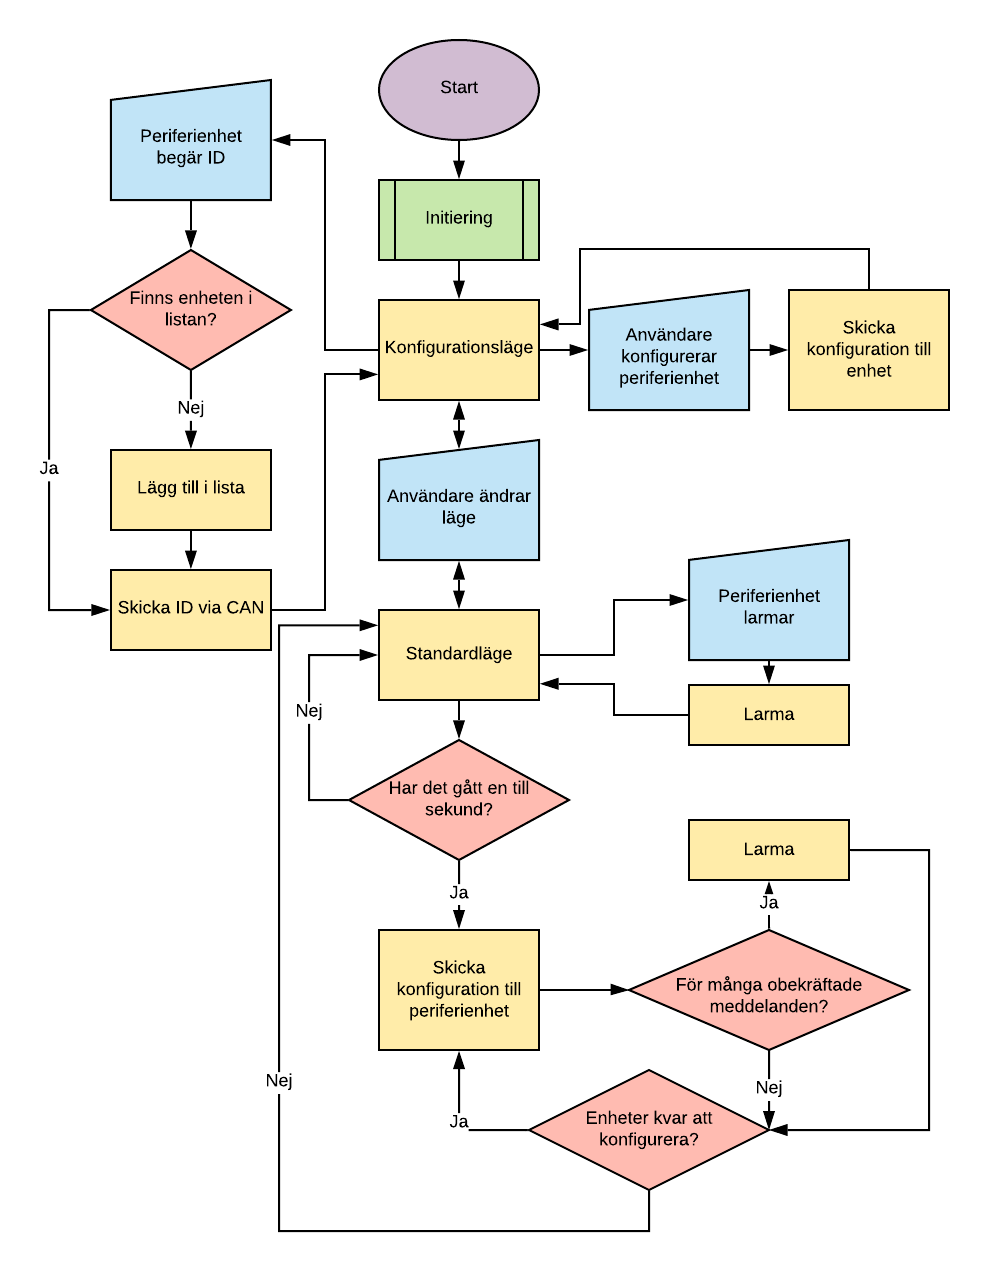
\includegraphics[scale=0.3]{figurer/Centralenhet.png}
    \caption{Flödesschema för centralenhetens viktigaste funktionalitet.}
    \label{fig:centralflöde}
\end{figure}

Centralenheten har följande två lägen:

\begin{description}
    \item[Startläge] Då centralenheten är i detta läge kan periferienheter ansluta sig till den genom att skicka en id-förfrågan via CAN, varpå centralenheten skickar tillbaka ett unikt id. Detta id används sedan för att adressera och identifiera periferienheten, se \ref{idbegäran} och \ref{idtilldelning}


    \item[Standardläge] Enheten väntar på larm-meddelanden från periferienheterna eller användarinput via USART. Dessutom skickar den regelbundet konfigurationen för anslutna dörrar och sensorer till periferienheterna, som förväntas bekräfta konfigurationen.
    Om en enhet inte svarar efter ett antal meddelanden går larmet.
\end{description}

I båda lägena kan användaren hantera periferienheterna genom konfigurationsändringar. För lösenordsskyddade kommandon används en knappsats som låter användaren logga in med en fyrsiffrig pinkod.


\subsubsection{Dörrenheten}
\label{subsec:Dörrenheten}
% Punkter att få med:
% - Systemuppstart
% - Lokala / Centrala Larm
% - CAN
% - Initiering?
% - Systick?
% - Bilder?

Dörrenheten är den periferienhet som sköter uppsikten över användarens dörrar. Enheten kräver en MD407-enkortsdator för drift.

För att koppla upp en dörr till systemet krävs det två anslutningar till en av mikrodatorns GPIO-portar: en koppling som går från en strömbrytare på dörren till en av mikrodatorns jämna I/O-pinnar (\textit{n}), samt en koppling från en LED-lampa på dörren till en udda I/O-pinne (\textit{n+1}).

Fyra av mikrodatorns fem portar är designerade för dörranslutningar (\textit{A,C,D,E}). \\
Eftersom samtliga portar har 16 tillgängliga pinnar innebär det att systemet maximalt kan stötta 32 dörrar per dörrenhet.

Port B är inte avsedd för dörranslutningar, utan används främst för CAN-\\kommunikationen
med centralenheten. En LED-lampa kan även kopplas till \\ pinne 2 på port B. Denna lampa signalerar vid vid uppstart när systemets initiering är färdig.

Vid uppstart initieras först portarna och pinnarna på mikrodatorn så att de kan adresseras
och avläsas på rätt sätt. Därefter startas en SystemTimer (SysTick) som fungerar som klocka för delsystemet.
Då klockan är startad initieras CAN på port B, vilket möjliggör kommunikation med centralenheten. Fortsättningsvis detekterar systemet hur många dörrar som är kopplade på kortet, och på vilka pinnar de är kopplade. För att dörrarna ska kunna detekteras krävs det att de är stängda.

Under detekteringen skapas datarepresentationer med förinställda värden för de dörrar som systemet
hittat. Efter att samtliga datarepresentationer är skapade kommer systemet att försöka kommunicera med centralenheten. Om en centralenhet inte svarar kommer systemet att gå in i lokal drift, vilket innebär att funktionaliteten med centrala larm uteblir.
Fortsättningsvis så tänds lamporna på dörrarna i den ordning som dess datarepresentationer skapades. Detta görs för att testa om de lokala larmen fungerar hos dörrarna. Efter att samtliga lampor är tända släcker systemet dem igen.
Slutligen tänds lampan som är kopplad till pinne 2 på port B för att signalera till användaren att enheten är redo för drift. Systemet kommer i fortsättningen kontinuerligt att skicka ut meddelanden till en eventuell centralenhet på CAN-nätverket med jämna mellanrum, vilket medför att en centralenhet kan kopplas in utan att systemet behöver startas om.

Systemet kontrollerar nu fortlöpande alla dörrar enligt flödesdiagrammet i figur \ref{fig:dörrflöde}:



\begin{figure}[H]
\begin{flushleft}
\end{flushleft}
\centering
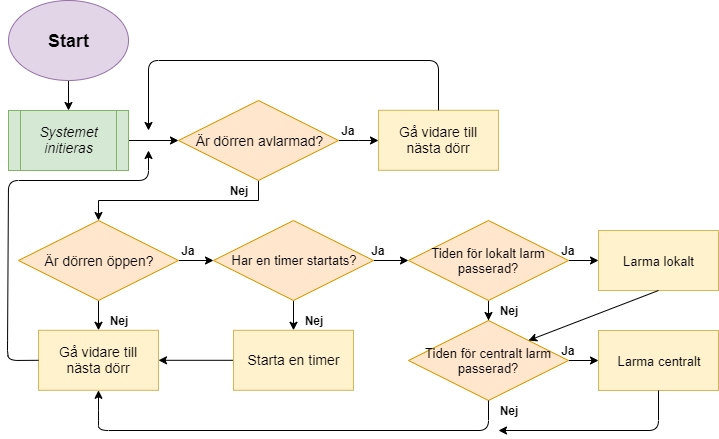
\includegraphics[scale=0.5]{figurer/Flow-Chart.png}
\caption{Flödesschema över dörrenhetens funktionalitet som visar vilka beslut systemet tar beroende på externa och interna händelser.}
\label{fig:dörrflöde}
\end{figure}

Dörrenhetens flöde bygger på polling. Samtliga dörrar har i sina datarepresentationer
ett antal kontrollbitar. I flödesschemat i figur 3 är dessa kontrollbitar representerade
som 'beslut' som anger huruvida en kontrollbit är satt till 1 (för \textit{ja}) eller 0
(för \textit{nej}). Dessa kontrollbitar sätts till 1 eller 0 beroende på externa händelser.

Avlarmning av en specifik dörr sker via CAN-kommunikation från centralenheten. Att en dörr är avlarmad
innebär att dess larm inte kan utlösas.

Att en dörr är öppen innebär att kretsen som går via strömbrytaren på dörren inte längre är sluten.
Om kretsen inte är sluten, och dörren inte är avlarmad, tyder det på att någonting externt har hänt
som systemet bör ta hänsyn till. Hur lång tid systemet väntar innan det larmar lokalt konfigureras i
 10-sekunders intervall via centralenheten. Väntetiden kan vara allt från 0 sekunder till ca 40 minuter
   (maxtiden är $2^8 *10$ sekunder).

När dörrenheten larmar centralt så skickas ett meddelande via CAN till centralenheten. Meddelanden
kommer skickas med intervall på en sekund tills centralenheten skickar tillbaka en ackreditering om att larmet har
 mottagits.

När dörrenheten larmar lokalt tänds en lampa på dörren. Detta larmet kan kompletteras med ett  ljudljud
genom att koppla in en högtalare på pinne A5 (port A, pinne 5). Ljudlarmet utlöses oavsett vilken dörr kopplad på enkortsdatorn som larmar. Användning av ljudlarmet sker på bekostnad av en dörr, då en dörr inte längre kan kopplas på A4-A5.


\subsubsection{Rörelseenheten}
Denna periferienhet använder avståndsmätare av modellen HC-SR04\cite{HC-SR04} till rörelsesensorer,
 och vibrationssensorer av modellen SW-18010P\cite{SW-18010P}, som styrs av ett MD407-enkortsdator.

Rörelseenheten använder fyra av enkortsdators fem GPIO-portar, port A, C, D och E.
Port B har många designerade pinnar till CAN med mera och är därför utesluten som
sensorport. Portarna är uppdelade mellan port A och C till rörelsesensorerna,
och port D och E till vibrationssensorerna. Dock har GPIO-port A har vissa designerade pinnar
till bland annat USART , därför går det ej att koppla sensorer till dessa (se tabell \ref{tab:Ogiltliga pinnar}).

\begin{table}[htbp]
	\centering
	\begin{tabular}{|c|c|} \hline
		GPIO-port & GPIO-pin \\ \hline \hline
		GPIOA & 1 \\ \hline
		GPIOA & 10 \\ \hline
		GPIOA & 13 \\ \hline
	\end{tabular}
	\caption{GPIO-pinnar på port A som ej går att koppla sensorer till.}
	\label{tab:Ogiltliga pinnar}
\end{table}

Vid uppstart initieras först portarna och pinnarna på mikrodatorn så de kan adresseras och avläsas på rätt sätt. Därefter startas en System Timer (SysTick) som används som klocka.
Fortsättningsvis detekterar systemet hur många rörelse- och vibrationssensorer som är inkopplade till kortet, och på vilka pinnar de är kopplade. För att vibrationssensorerna skall detekteras får de ej utsättas för vibrationer under uppstart.

Efter detekteringen skapas datarepresentationer med förinställda värden för de
sensorer som systemet hittat. Efter att samtliga datarepresentationer är skapade skickas
en lista av de inkopplade sensorerna till centralenheten som bestämmer vilka sensorer som ska vara aktiva
samt sätter centrala och lokala larmavståndet för rörelsesensorerna.

Systemet itererar nu över alla inkopplade sensorer enligt figur \ref{fig:MotionFlow}. \newpage


\begin{figure}
\centering
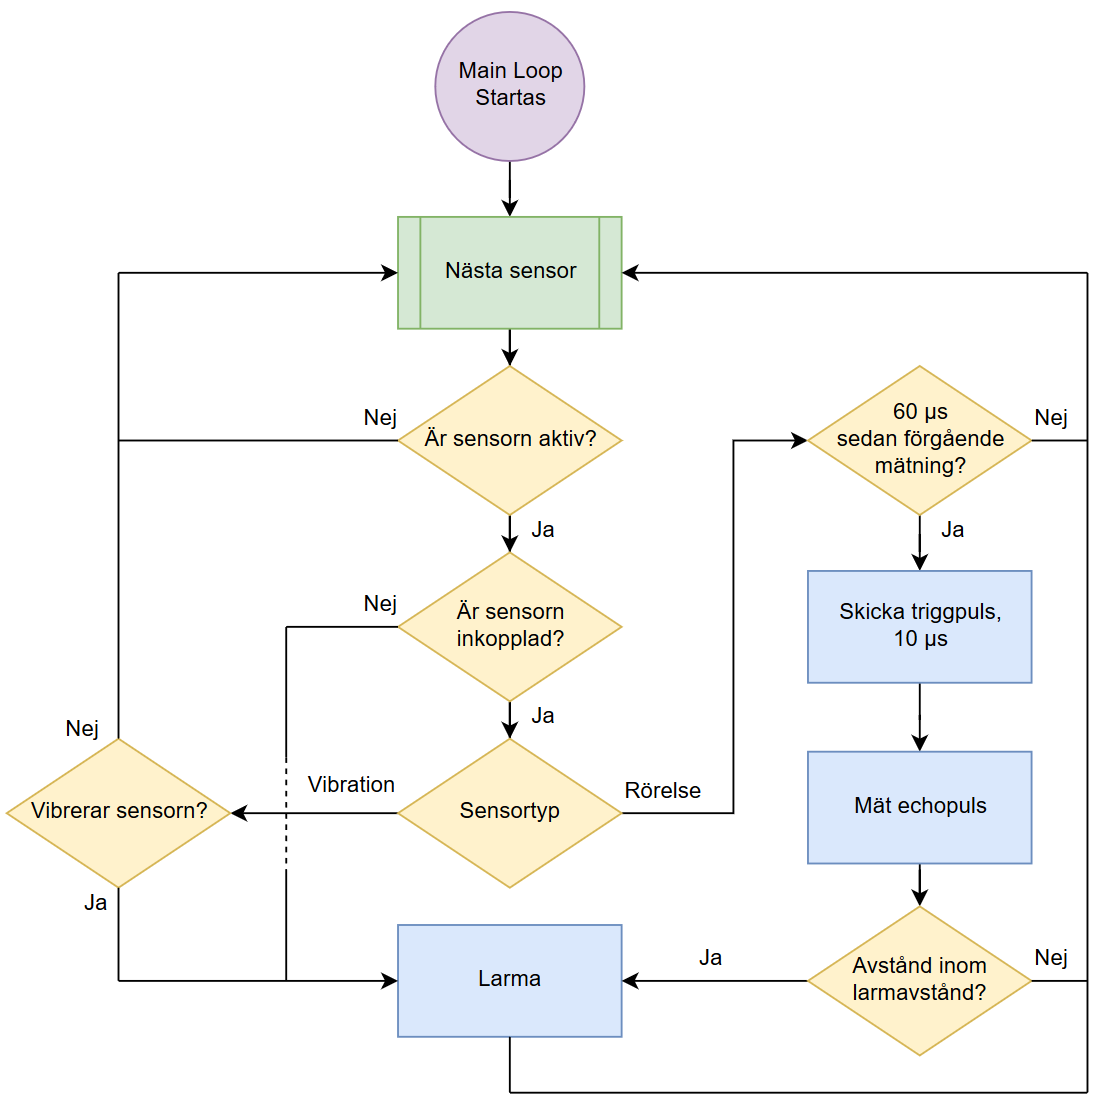
\includegraphics[scale=0.3]{figurer/FlowchartMotion.png}
\caption{Flödesschema över rörelseenheten.}
 \label{fig:MotionFlow}
\end{figure}

Rörelseenhetens flöde bygger på polling. Polling är smidigt då avståndsmätarna skickar och tar emot pulser av olika längd
och behöver då ha timers som håller koll på detta. Ifall detta hade skett via fördröjningsfunktioner hade alla andra sensorer
inte fungerat under pulsmätningar och en säkerhetsrisk skulle uppstå. Avbrottshantering är en annan lösning på problemet,
men då alla sensorer prioriteras lika är polling den simplare lösningen.


\textbf{Rörelsesensorn}:
En rörelsesensor tar upp 3 pinnar och får därmed plats med 5 rörelsesensorer per port.
Trig- och echo-pinnen från HC-SR04 samt en LED-lampan kopplas resepktive till  pin-\textit{n}, -$(n+1)$ och -$(n+2)$.


Sensorn aktiveras genom att MD407-enkortsdatorn skickar en hög puls till sensorn i minst 10 mikrosekunder,
varpå sensorn skickar ut ultraljudsvågor och sänder en hög puls till MD407-enkortsdatorn fram tills ultraljudsvågorna har återvänt.
Avståndet till närmaste föremål beräknas genom att mäta längden på pulsen. HC-SR04 kan mäta avstånd upp till 400 cm.

Rörelsesensorn har både centralt och lokalt larm. Avståndet för centrala larmet ställs in av centralenheten via CAN-kommunikation
upp till 400 cm. När det centrala larmet går skickas ett CAN-meddelande till centralenheten som agerar därefter.
Avståndet för lokala larmet sätts automatiskt till två gånger det centrala larmavståndet. Ifall centrala larmsvtåndet är över 200 cm kommer
lokala larmavståndet sättas till 400. När det lokla larmet går tänds en LED-lampa tills sensorn inte längre känner av något inom
det lokala larmavståndet.

\textbf{Vibrationssensorn}:
En vibrationssensor tar upp 2 pinnar och får därmed plats med 8 vibrationssensorer per port.
En pinne för digital-ouput från SW-18010P och en LED-lampa kopplas till pin-\textit{n} respektive pin-$(n+1)$.

Sensorn sänder kontinuerligt en hög puls till MD407-enkortsdatorn utom när den
känner av vibrationer, då den istället sänder en låg puls. Sensorns känslighet justeras fysiskt genom en komparator på sensorn.
Vibrationssensorn har endast central larm som skickas via CAN.

\newpage
 \section{Resultat}
 För kompletta testspecifikationer hänvisas till bilaga \ref{bilaga:tester}.

 % Detta avsnitt redovisar resultatet av genomförd verifirering av systemet; dels fördelarna, dels för komplett system. Detta avsnitt redovisar även resultatet av det slutgiltiga fysiska testet när hela systemet körs i skarpt läge. Ni ska främst redovisa resultat i form av funktionalitet, men ta ocks upp prestanda aspekter om dessa är viktiga. Diskutea hur väl ni lyckats med er slutprodukt i förhållande till er projektplan.
 \subsection{Larmsystemet som helhet}

 Larmsystemet fyller all funktionalitet som beskrevs i projektplaneringen.
 Systemet som testats har bestått av en dörrenhet, en rörelseenhet, och en centralenhet.
 Det har även testats att ha en störenhet kopplad till systemet, för att testa systemet mot brusmeddelanden.
 Kommunikationen mellan enheterna fungerar och har skett via en CAN-buss som planerat.

 Periferienheterna har funktionaliteten att larma både lokalt och centralt, och kan ta emot konfigurationer till sensorerna från centralenheten. Ifall en periferienhet inte svarar på centralenhetens regelbundna konfigurationsmeddelande larmas det centralt, detta för att säkerställa att enheter inte kopplas ur systemet.

 Tester visar med god säkerhet att larmmeddelanden når centralenheten även med mycket brus på CAN-bussen. Tester har även visat att centralenheten kan hantera att skicka stora mängder meddelanden utan att något meddelande förloras.
 När en sensor på en enhet begär ett centralt larm fortsätter den att larma tills att centralenheten har skickat ett avlarmningsmeddelande.
 Ifall en enhet larmar centralt men inte ackrediterats skickas ett nytt larm för att säkerställa att centralenheten hanterar larmet.

 Efter att återspelningsenheten testats så att den fungerar som förväntat (se bilaga \ref{test:replayer}) så testades systemet mot återuppspelningsattacker (se bilaga \ref{test:sessionID}). Detta visade att systemet med hjälp av sessions-id klarar av att förhindra återuppspelningsattacker. Det faktum att återspelaren lyckades begära ett id har den enkla förklaring att meddelanden inte filtreras på sessions-id innan id-tilldelningen är färdig (se bilaga \ref{bilaga:protokoll}).

 \subsection{Centralenheten}
 Centralenheten har följande funktionalitet:
 \begin{enumerate}
     \item Tilldelning av id till periferienheter.
     \item Konfiguration av periferienheter via USART.
     \item Automatisk detektering av enheter som lämnar nätverket.
     \item Larmhantering.
 \end{enumerate}

 \begin{itemize}
\color{white}
\item Abra kadabra blankrad!
\end{itemize}

 För att säkerställa ovan nämnda funktionalitet utfördes följande tester:
 \begin{enumerate}
     \item Test av id-begäran och larmmeddelnade, se bilagor \ref{test:UrkopplingMotion} och \ref{test:idLarm}.
     \item Konfigurering av rörelseenhet, se bilaga \ref{test:MotionConfig}
\end{enumerate}

Utöver ovan nämnda tester är centralenheten involverad i alla de testar som inkluderar kommunikation mellan enheter. Även i de systemövergripande testerna (\ref{test:brusTest} och \ref{test:replayer}) har centralenheten presterat som förväntat. Centralenheten har klarat att kommunicera med periferienheter trots mycket trafik på CAN-bussen och även förhindrat återuppspelningsattack genom sessions-id. Allt som allt klarar centralenheten det som förväntas. Dock skulle  ett mer användarvänligt kommandogränssnitt vara önskvärt då det nuvarande kan upplevas som klumpigt.



 \subsection{Dörrenheten}

Dörrenheten har följande funktionalitet:
 \begin{enumerate}
     \item Detektering av antalet stängda dörrar kopplade på enkortsdatorn.
     \item Signalering via LED-lampa som indikerar att dörrenhetens initiering är färdig.
     \item Lokal larmning via LED-lampa och ljud.
     \item Central larmning via CAN-buss.
     \item Går att konfiguera väntetider innan larm från centralenheten.
     \item Avlarmning av individuella dörrar från centralenheten.
     \item Dörrar kan konfigueras ifrån centralenheten.
     \item Lokal funktionalitet kräver inte uppkopplad centralenhet.
     \item Stöd för 32 dörrar.
 \end{enumerate}


 \begin{itemize}
\color{white}
\item Hokus pokus jag har tappat mitt fokus.
\end{itemize}

 För att säkerställa att funktionalitet ovan fungerar utfördes följande tester:
 \begin{enumerate}
     \item Test av pinnar för dörrar \ref{test:portTest}
     \item Test av lokal drift \ref{test:localDrift}
     \item Test av id-tilldelning och larm \ref{test:idLarm}
     \item Test av system med brus \ref{test:brusTest}
     \item Test av återuppspelningsattack \ref{test:replayer}
 \end{enumerate}

 \subsection{Rörelseenheten}

Rörelseenheten klarar att hantera ett flertal vibrations- och rörelsesensorer samtidigt, upp till 23 sensorer,
och möjligheten att koppla upp flera rörelseenheter till samma centralenhet finns.

Rörelseenheten har följande funktionalitet:
 \begin{enumerate}
 	\item Automatiskt detektera antalet inkopplade rörelse- och vibrationssensorer vid uppstart.
	\item Larma vid upptäckt av vibrationer, rörelse och urkoppling av aktiv sensor.
    \item Central larmning via CAN-buss.
	\item Avlarmning via centralenheten.
	\item Lokal larmning för rörelsesensorer via LED-lampa.
	\item Konfigurerbara larmvillkor från centralenheten.
	\item Avaktivering av sensorer.
	\item Kalibrering av rörelsesensorerna via centralenheten.
 \end{enumerate}

 \begin{itemize}
\color{white}
\item Sim sala bim, nu är det radbyte!
\end{itemize}

 För att säkerställa att funktionalitet ovan fungerar utfördes följande tester:
 \begin{enumerate}
	\item Test av portar samt lokalt och centralt larm för rörelseenheten.\ref{test:PortMotion}
	\item Konfiguration och kalibrering av rörelseenheten.\ref{test:MotionConfig}
	\item Urkopplingslarm rörelseenheten.\ref{test:UrkopplingMotion}
	\item Prestandatest rörelseenheten.\ref{test:MotionPrestanda}
 \end{enumerate}

\newpage
\section{Diskussion och slutsats}
% Detta avsnitt innehåller en sammanfattning av konstruktionen och en diskussion av resultatet. Om detta är möjligt, dra slutsatser av ert projekt och identifiera förbättringsmöjligheter. (Vilka kan vara användbara för en beställare)

Tidigt i projektets gång var vi tvungna att välja mellan polling eller avbrott för att respondera på externa händelser för dörr- och rörelseenheten.  Polling valdes dels för att koden blir lättare att först och lättare att underhålla, men även för att tanken med systemet är att inget larm ska ha högre prioritet än något annat. 

Skulle dörrenhetens mjukvara utvecklats med avbrott hade den enda fördelen varit möjligheten att dela upp dörrarna så att de hade olika prioritet på CAN-bussen, vilket skulle kunna resultera i att vissa larm skulle kommit fram till centralenheten snabbare än de hade med polling. 
Tiden man tjänar in handlar om millisekunder, och eftersom MD407-enkortsdatorn endast stöttar 16 avbrottslinor skulle det ändå behövas  någon form av polling ifall systemet ska ha mer än 16 dörrar. 
Prestandatestet som utfördes visade inte på någon märkbar fördröjning, så valet med polling känns högst befogat, se bilaga \ref{test:prestandaTest}

Polling har även använts till stor fördel inom rörelseenheter, med hjälp av polling kan flera rörelsensorer mätas av samtidigt, då det inte behövs blockerande väntetid-funktioner för att mäta/vänta en specifik tid. 
Uppoffringen som görs är precision, med ett polling system är det svårt att vänta exakta tider, då det endast kollas ifall en tidsvariabel har överstigit en annan, och det går lite tid mellan att dessa villkor kollas.
Denna tid är dock såpass liten och skillnader i väntetider är såpass osignifikanta att det inte påverkar systemets funktionalitet, se bilaga \ref{test:MotionPrestanda}.


Samtliga delsystem har uppnått de grundkraven som formulerades i målsättningen, men även utrustats med
ytterligare funktionalitet som varit naturlig att implementera under projektets gång. Rörelse- och dörrenheten
kan ha upp till 23 respektive 32 sensorer och centralenheten kan ha upp till 32 periferienheter.
Med denna information kan vi dra slutsatsen att ett skalbart larmsystem är uppnåt.
% Referenser enligtIEEE.
%För referenser
\bibliographystyle{IEEEtran}
\bibliography{referenser}

% Avslutningsvis så vill vi påminna om att projektets slutrapport, precis som projektplanen, ska vara projektintern, det väl säga att den ska beskriva det tekniska utvecklingsarbetet och bortse från att projektarbetet faktiskt organiserats inom ramen för en kurs.

\appendix
    \section{Utförlig beskrivning av meddelandetyper kommunikationsprotokoll}
    \label{bilaga:protokoll}
        \section*{Grundidé}
\label{sec:grundide}

Centralenheten sparar all status och datainformation, denna information kopieras regelbundet till perferienheterna via konfigureringsmeddelanden. Centralenheten har 2 lägen.

\begin{enumerate}
	\item Standard running. Här lyssnar man på larm från periferienheterna. Dessutom skickar man regelbundet  konfigurationen för anslutna dörrar och sensorer. Periferienheten svarar ok, om den inte svarar efter ett antal meddelande larmar man.
	\item Vid uppstart är centralenheten i konfigurationsläge. Nu kan man via USART konfigurera anslutna dörrlarmsenheter samt lörelselarm.
\end{enumerate}

Varje perferienhet förväntas ha en unik fysisk adress som kommer användas vid tilldelning av ID adresser. Likt fysiska MAC adresser och logiska IP adresser i ethernet.

\section*{Bitfördelning i identifieringsdelen av meddelandet}
\label{sec:bitfördelning}

Totalt 11 bitar (Utan att utöka med 18 bitar till)
\begin{description}
	\item{0-2:} Första bitarna är meddelandetyp. 3 bitar dvs 8 meddelandetyper.
	\item{3:} en bit för riktning. Från/till centralenheten. Kan ses som en 4e bit i meddelandetypen.
	\item{4-10:} 7 bitar:
		Om riktning är till centralenheten är bitarna sändarens ID.
		Om riktningen är från centralenheten beskriver bitarna mottagarens ID.
		Innan enheten har en egen ID används bara ettor.
\end{description}


\section*{Meddelandetyper lista}
\label{sec:meddelandetyper}

\begin{table}[H]
	\begin{tabular}{|c|l|p{2.6cm}|p{6cm}|}
		\hline
		N& Riktning & Meddelandenamn & Beskrivning \\ \hline \hline
		0 & p -> c & Ack & Acknowledgement för senaste meddelandet. \\ \hline
		1 & p -> c & Skicka larm & Talar för centralenheten om någon dörr eller sensor larmar. \\ \hline
		3 & Båda & Skicka konfiguration & Skickar konfiguration till periferienheten kontinuerligt. Fungerar även som ping. Perferienheterna skickar sina konfigurationener i andra riktingen vid uppstart. Rörelselarmet har mätvärden i denna typ av meddelande. \\ \hline
		4 & c -> p & Tilldelning av ID & Centralenheten tilldelar en periferienhet dess ID. Enheten identifieras med dess fysiska adress i meddelandet. Detta meddelande skickas bara då centralenheten är i konfigurationsläge (läge  2). \\ \hline
		5 & p -> c & Ny enhet här & Centralenheten tilldelar en periferienhet dess ID. Enheten identifieras med dess fysiska adress i meddelandet. Detta meddelande skickas bara då centralenheten är i konfigurationsläge (läge  2). \\ \hline
	\end{tabular}
	\label{tab:meddelandetyper}
\end{table}

\section*{Detaljinformation angående meddelandetyperna}
\label{sec:detaljinfo}
\textbf{Skicka konfiguration} \\
I datadelen av meddelande för dörrlarm borde det finnas:
\begin{itemize}
	\item Ett par bitar för addressen till dörren i fråga.
	\item En aktiveringsbit per dörr.
	\item En bit per dörr för avaktivering av pågående larm.
	\item Ett par bitar för varje tidsfördröjning.
\end{itemize}

I datadelen av meddelande för rörelsesensorlarm borde det finnas:
\begin{itemize}
	\item En aktiveringsbit per sensor
	\item En bit per sensor för avaktivering av pågående larm.
	\item En bit per enhet för aktivering av automatisk översändning av “Skicka larm och mätvärden” meddelanden. Detta kommer användas vid konfiguration av avståndsgivare.
\end{itemize}

\section*{Todo}
\label{sec:todo}
Borde man ha olika meddelandetyper för “Skicka larm” beroende på vilken enhetstyp det rör sig om?


    \section{Kommandolista för centralenheten}
    \label{kommandon}
        För att styra centralenheten används ett antal kommandon som beskrivs nedan.

    \textbf{start}\\
    Startar standardläge.

    \textbf{list}\\
    Skriver ut alla periferienheter i terminalen och anger varje sensors konfiguration. Detta kommando används med fördel för att ta reda på vilka värden som är lämpliga för kommandona dor och ror (se nedan).

    \textbf{dor v x y z}\\
    Där \textbf{v, x, y} och \textbf{z} är tal mellan 0 och 9. Konfigurerar dörr \textbf{x} på enhet med id \textbf{v} med timer för lokalt larm på  \(\textbf{y} * 10\) sekunder samt en fördröjning till centralt larm på \(\textbf{z} * 10\) sekunder.

    \textbf{ror x y z}\\
    Där \textbf{x, y} och \textbf{z} är tal mellan 0 och 9. Konfigurerar rörelsesensor \textbf{y} på enhet med id \textbf{x} för att larma då den detekterar ett föremål på ett avstånd mindre än \(\textbf{z} * 10\) centimeter.

    \textbf{avlarma y z} \\
    Avlarmar sensor \textbf{z} på rörelseenhetenhet med id \textbf{y}. Detta kommando är lösenordsskyddat.

    \textbf{larma y z} \\
    Larmar sensor \textbf{z} på rörelseenhet med id \textbf{y}. Alla sensorer är larmade som standard så detta kommando körs om man vill återaktivera larm efter att det avaktiverats. Detta kommando är lösenordsskyddat.

    \textbf{inak y z} \\
    Inaktiverar sensor \textbf{z} på enhet med id \textbf{y}. Detta kommando är lösenordsskyddat.

    \textbf{ak y z} \\
    Aktiverar sensor \textbf{z} på enhet med id \textbf{y}. Alla sensorer är aktiverade som standard så detta kommando körs om man vill återaktivera en sensor efter att den inaktiverats. Detta kommando är lösenordsskyddat.

    \textbf{kal x y z} \\
    Startar översändning av kalibreringsmeddelanden till rörelsesensor \textbf{y} på rörelseenhet med id \textbf{x}. Det upplätta avståndet för givaren är \(\textbf{z} * 10\). Kalibrering fungerar inte om sensorn är inaktiverad.

    \textbf{nokal y z} \\
    Avslutar översändning av kalibreringsmeddelanden för sensor \textbf{z} på enhet \textbf{y}.


	\clearpage
	\section{Tester}
    		\label{bilaga:tester}
     	%Beskrivande titel av testet samt en unik label
\subsection{Test av pinnar för dörrar}
\label{test:portTest}

\setlength{\columnsep}{1cm}


% Vid utförande av test fylls mallen nedan i, vilket resulterar i ett protokoll som sedan sparas som verifikation. Målet med dessa protokoll är att man utan sakkunskap ska kunna skapa sig en överblick av att systemet fungerar som det ska.


\begin{multicols}{2}
\subsubsection*{Test formulerat av}
% Namn på den/de som formulerade testet.
Adam

\subsubsection*{Utfört av}
% Namn på den/de som utförande testet.
Filip


\end{multicols}
\subsubsection*{Komponent}
%Vilken del av systemet testas?
Dörrenheten


\subsubsection*{Testsyfte}
%Vad ska testet visa? Är testet till följd av tidigare test?
Säkerställa att alla portar fungerar.


\subsubsection*{Hjälpmedel}
%Lista hjälpmedlen som användes i samband med testet.
\begin{itemize}
	\item Ledlampor
	\item Dörrbrytare
	\item Kopplingskapel
	\item kopplingsbräda
\end{itemize}



\subsubsection*{Utförande}
%Hur ska testet utföras?
Testa portarna A, C, D och E  en åt gången genom att koppla in dörrbrytare på pinnar med jämt index (0,2,4..) och tillhörande ledlampor på pinnarna ovanför (1,3,5..). Kör sedan programkoden för dörrenheten och vänta tills initsieringen är utförd och programet är i lokal drift. Ta nu bort magneten från dörrbrytaren och kontrollera så att tillhörande lampa tänds.


\subsubsection*{Resultat}
%Vad är testresultatet? Hittades några buggar?
Lamporna tänds som dem ska.



\subsubsection*{Analys}
%Vad innebär testets resultat? Behövs fler test av komponenten? Behöver andra komponenter testas ytterligare, och i så fall hur?
De använda portarna fungerar som dem ska.



	\clearpage
%Beskrivande titel av testet samt en unik label
\subsection{Test av portar samt lokalt och centralt larm för rörelseenheten}
\label{test:PortMotion}

\setlength{\columnsep}{1cm}


% Vid utförande av test fylls mallen nedan i, vilket resulterar i ett protokoll som sedan sparas som verifikation. Målet med dessa protokoll är att man utan sakkunskap ska kunna skapa sig en överblick av att systemet fungerar som det ska.


\begin{multicols}{2}
\subsubsection*{Test formulerat av}
% Namn på den/de som formulerade testet.
Erik

\subsubsection*{Utfört av}
% Namn på den/de som utförande testet.
Adam


\end{multicols}
\subsubsection*{Komponent}
%Vilken del av systemet testas?
Rörelseenheten


\subsubsection*{Testsyfte}
%Vad ska testet visa? Är testet till följd av tidigare test?
Säkerställa att sensorer kan kopplas in på rörelseenhetens alla portar samt testa ifall både lokalt och centralt larm fungerar.

\subsubsection*{Hjälpmedel}
%Lista hjälpmedlen som användes i samband med testet.
\begin{itemize}
	\item Avståndsmätare, HC-SR04
	\item Vibrationssensor, SW-18010P
	\item CAN-kabel
	\item Kopplingskabel
	\item Kopplingsbräda
	\item LED-lampor
\end{itemize}



\subsubsection*{Utförande}
%Hur ska testet utföras?
Testa portarna A, C, D och E genom att koppla en rörelsesensor till port A och en till C samt en vibrationssensor till D och en till E. För rörelsesensorerna kopplas HC-SR04:s trigpin till en pinne på MD407-mikrodatorn som uppfyller 3n (0,3,6.. o.s.v.), HC-SR04:s echopin till pinne (3n + 1) och LED-lampa till pinne (3n + 2). 
För vibrationssensorn kopplas SW-18010P:s DO-pinne till en pinne på MD407-mikrodatorn som uppfyller 2n(0,2,4.. o.s.v.) samt en LED-lampa till pinne (2n + 1). 
se till att rörelseenheten är kopplad  till centralenheten via CAN kabel. Starta centralenheten och håll den i 'startläge', starta nu rörelseenheten och kolla att centralenheten hittar en rörelsesensor på rörelseenheten. Sätt nu centralenheten i 'standardläge' så att den skickar standardkonfigurationer till rörelseenheten, 20 respektive 40 cm centralt och lokalt larmavstånd. Verifiera att LED-lampan till rörelsesensorn börjar lysa när du håller handen ca 30 cm från sensorn. Verifiera sedan att sensorn skickar larm till centralenheten när du håller handen närmare än 20 cm ifrån. Peta på vibrationssensorn och kolla ifall centralenheten får larm.

\subsubsection*{Resultat}
%Vad är testresultatet? Hittades några buggar?
Alla LED-lampor lyste och centralenheten fick larm för både rörelse- och vibratoinssensorn.


\subsubsection*{Analys}
%Vad innebär testets resultat? Behövs fler test av komponenten? Behöver andra komponenter testas ytterligare, och i så fall hur?
Alla rörelseenhetens portar samt lokalt och centralt larm fungerar som de ska.



	\clearpage
%Beskrivande titel av testet samt en unik label
\subsection{Konfiguration och kalibrering av rörelseenheten}
\label{test:MotionConfig}

\setlength{\columnsep}{1cm}


% Vid utförande av test fylls mallen nedan i, vilket resulterar i ett protokoll som sedan sparas som verifikation. Målet med dessa protokoll är att man utan sakkunskap ska kunna skapa sig en överblick av att systemet fungerar som det ska.


\begin{multicols}{2}
\subsubsection*{Test formulerat av}
% Namn på den/de som formulerade testet.
Erik

\subsubsection*{Utfört av}
% Namn på den/de som utförande testet.
Filip


\end{multicols}
\subsubsection*{Komponent}
%Vilken del av systemet testas?
Rörelseenheten


\subsubsection*{Testsyfte}
%Vad ska testet visa? Är testet till följd av tidigare test?
Säkerställa att konfigurationsmeddelanden och kalibrering från centralenheten fungerar.

\subsubsection*{Hjälpmedel}
%Lista hjälpmedlen som användes i samband med testet.
\begin{itemize}
	\item Avståndsmätare, HC-SR04
	\item Vibrationssensor, SW-18010P
	\item Kopplingskabel
	\item Kopplingsbräda
	\item LED-lampor
\end{itemize}



\subsubsection*{Utförande}
%Hur ska testet utföras?
Koppla upp rörelseenheten till centralenheten och ha en rörelsesensor och en vibrationssensor inkopplad. Skicka konfiguration från centralenheten som säger att de båda sensorerna ska vara aktiva och sätt larmavståndet för rörelsesensorn till 20 cm. Testa nu att utlösa sensorernas larm. Avlarma sedan båda sensorerna. Inaktivera nu de båda sensorerna från centralenheten och verifiera att du ej längre kan larma dem. Aktivera nu rörelsesensorn igen. 
Håll nu ett objekt 40 cm ifrån rörelsesensorn och kalibrera sensorn via centralenheten genom att skicka kalibreringsvärdet 20 cm. Rör sedan obejktet några centimeter närmare och verifiera att rörelsesensorn larmar.


\subsubsection*{Resultat}
%Vad är testresultatet? Hittades några buggar?
Konfigurering, larmning samt avlarmning fungerade som förväntat. Vid kalibrering var det svårt att hålla reda på kommandona men när det väl löste sig så gick kalibreringen bra och sensorn larmade på ett onaturligt långt avstånd precis som förväntat.



\subsubsection*{Analys}
%Vad innebär testets resultat? Behövs fler test av komponenten? Behöver andra komponenter testas ytterligare, och i så fall hur?
Konfigurering samt kalibrering fungerar för rörelsesensorn. Kommandohanteringen skulle kunna göras enklare underlätta för användaren.



	\clearpage
%Beskrivande titel av testet samt en unik label
\subsection{Urkopplingslarm rörelseenheten}
\label{test:UrkopplingMotion}

\setlength{\columnsep}{1cm}


% Vid utförande av test fylls mallen nedan i, vilket resulterar i ett protokoll som sedan sparas som verifikation. Målet med dessa protokoll är att man utan sakkunskap ska kunna skapa sig en överblick av att systemet fungerar som det ska.


\begin{multicols}{2}
\subsubsection*{Test formulerat av}
% Namn på den/de som formulerade testet.
Erik

\subsubsection*{Utfört av}
% Namn på den/de som utförande testet.
Filip


\end{multicols}
\subsubsection*{Komponent}
%Vilken del av systemet testas?
Rörelseenheten


\subsubsection*{Testsyfte}
%Vad ska testet visa? Är testet till följd av tidigare test?
Säkerställa att aktiva sensorer som kopplas ur larmar.

\subsubsection*{Hjälpmedel}
%Lista hjälpmedlen som användes i samband med testet.
\begin{itemize}
	\item Avståndsmätare, HC-SR04
	\item Vibrationssensor, SW-18010P
	\item CAN-kabel
	\item Kopplingskabel
	\item Kopplingsbräda
	\item LED-lampor
\end{itemize}



\subsubsection*{Utförande}
%Hur ska testet utföras?
Dra ut valfri kopplingskabel från en avståndsmätare och en vibrationssensor medan rörelseenheten är underdrift och centralenheten konfigurerat dessa sensorer till aktiva.
Kontrollera att sensorerna larmar till centralenheten vid urkoppling.


\subsubsection*{Resultat}
%Vad är testresultatet? Hittades några buggar?
Larmeddelande skickades för respektive sensor skickades till centralenheten när de kopplades ur.


\subsubsection*{Analys}
%Vad innebär testets resultat? Behövs fler test av komponenten? Behöver andra komponenter testas ytterligare, och i så fall hur?
Går ej att kringå rörelseenhetens larm genom att koppla ur dess sensorer.



	\clearpage
%Beskrivande titel av testet samt en unik label
\subsection{Prestandatest rörelseenheten}
\label{test:MotionPrestanda}

\setlength{\columnsep}{1cm}


% Vid utförande av test fylls mallen nedan i, vilket resulterar i ett protokoll som sedan sparas som verifikation. Målet med dessa protokoll är att man utan sakkunskap ska kunna skapa sig en överblick av att systemet fungerar som det ska.


\begin{multicols}{2}
\subsubsection*{Test formulerat av}
% Namn på den/de som formulerade testet.
Erik

\subsubsection*{Utfört av}
% Namn på den/de som utförande testet.
Gustav


\end{multicols}
\subsubsection*{Komponent}
%Vilken del av systemet testas?
Rörelseenheten


\subsubsection*{Testsyfte}
%Vad ska testet visa? Är testet till följd av tidigare test?
Säkerställa att ingen märkbar fördröjning sker vid flera inkopplade rörelsesensorer.

\subsubsection*{Hjälpmedel}
%Lista hjälpmedlen som användes i samband med testet.
\begin{itemize}
	\item Avståndsmätare, HC-SR04
	\item CAN-kabel
	\item Kopplingskabel
	\item Kopplingsbräda
\end{itemize}



\subsubsection*{Utförande}
%Hur ska testet utföras?
Koppla först upp en rörelsesensor till rörelseenheten och koppla upp rörelseenheten till centralenheten via CAN. Starta programmen och skicka standard konfiguration på 20 cm larmavsttånd från centralenheten till rörelsesensorn. Testa att sensorn larmar på 20 cm. Starta nu om och koppla upp fyra extra rörelsesensorer. Testa ifall första sensorn som testades fortfarande larmar på 20 cm. Sensorn ska vara okalibrerad för att inte fuska fram samma värde båda gångerna.

\subsubsection*{Resultat}
%Vad är testresultatet? Hittades några buggar?
Sensorn larmade första gången 20.5 cm bort och larmade på samma avstånd efter det kopplats in 4 till rörelsesensorer.


\subsubsection*{Analys}
%Vad innebär testets resultat? Behövs fler test av komponenten? Behöver andra komponenter testas ytterligare, och i så fall hur?
Gick ej att se skillnad på larmavstånd när flera rörelsesensorer, som tar upp större delen av kod exekveringen, är inkopplade. Alltså kan vi dra slutsatsen att rörelseenheten klarar av att exekvera kod för flertalet sensorer samtidigt utan några problem. Även om larmavståndet ändrats med några procent hade detta fixats av kalibrering.



         \clearpage
%Beskrivande titel av testet samt en unik label
\subsection{Test av ID-tilldelning och larm}
\label{test:idLarm}

\setlength{\columnsep}{1cm}


% Vid utförande av test fylls mallen nedan i, vilket resulterar i ett protokoll som sedan sparas som verifikation. Målet med dessa protokoll är att man utan sakkunskap ska kunna skapa sig en överblick av att systemet fungerar som det ska.


\begin{multicols}{2}
\subsubsection*{Test formulerat av}
% Namn på den/de som formulerade testet.
Adam och Filip

\subsubsection*{Utfört av}
% Namn på den/de som utförande testet.
Erik


\end{multicols}
\subsubsection*{Komponent}
%Vilken del av systemet testas?
Centralenhet och dörrenhet



\subsubsection*{Testsyfte}
%Vad ska testet visa? Är testet till följd av tidigare test?
Kontrollera att dörrenheten blir tilldelad ett ID av centralenheten vid uppstart. Därefter ska dörrenheten larma om dörrbrytaren bryts.


\subsubsection*{Hjälpmedel}
%Lista hjälpmedlen som användes i samband med testet.
\begin{itemize}
	\item CAN-kabel
	\item Dörrbrytare
	\item kopplingskabel
	\item CAN-lyssnare
\end{itemize}



\subsubsection*{Utförande}
%Hur ska testet utföras?
Koppla upp en dörrbrytare på en port (A, C, D eller E). Därefter kopplas CAN-nätverket upp med lyssnare, centralenhet och dörrenhet. Starta sedan lyssnaren och centralenheten. Se till att centralenheten är i konfigurationsläge och starta därefter dörrenheten. Kontrollera nu att ID-tilldelningen sker genom att kolla på kommunikationen som lyssnare detekterar samt utskriften från centralenheten. 

Efter ID-tilldelningen är färdig sätts centralenheten i standarsläge genom att skriva kommandot start i konsolen. Testa nu att centralenheten detekterar larm som skickas från dörrenheten då dörrbrytaren öppnas. Läs första byten av meddelandet, här skickas ID till dörrenheten och ska vid detta läge vara 0.

Starta om dörrenheten och utför samma test igen. Denna gång ska IDt vara 1.


\subsubsection*{Resultat}
%Vad är testresultatet? Hittades några buggar?
ID-tilldelningen sker som den ska. Larmet skickas efter ett par sekunder efter att dörrbrytaren öppnats och mottas av centralenheten med en utskrift i konsolen.


\subsubsection*{Analys}
%Vad innebär testets resultat? Behövs fler test av komponenten? Behöver andra komponenter testas ytterligare, och i så fall hur?
ID-tilldelningen utförs korrekt och dörrenheten kan därefter larma om en öppen dörrbrytare detekterats.



         \clearpage
%Beskrivande titel av testet samt en unik label
\subsection{Test av lokal drift för dörrenhet}
\label{test:localDrift}

\setlength{\columnsep}{1cm}


% Vid utförande av test fylls mallen nedan i, vilket resulterar i ett protokoll som sedan sparas som verifikation. Målet med dessa protokoll är att man utan sakkunskap ska kunna skapa sig en överblick av att systemet fungerar som det ska.


\begin{multicols}{2}
\subsubsection*{Test formulerat av}
% Namn på den/de som formulerade testet.
Adam

\subsubsection*{Utfört av}
% Namn på den/de som utförande testet.
Erik


\end{multicols}
\subsubsection*{Komponent}
%Vilken del av systemet testas?
Dörrenheten


\subsubsection*{Testsyfte}
%Vad ska testet visa? Är testet till följd av tidigare test?
För att säkerställa att dörrenheten körs lokalt ifall ingen central enhet hittas.


\subsubsection*{Hjälpmedel}
%Lista hjälpmedlen som användes i samband med testet.
\begin{itemize}
	\item Ledlampor
	\item Dörrbrytare
	\item Kopplingskapel
	\item kopplingsbräda
\end{itemize}



\subsubsection*{Utförande}
%Hur ska testet utföras?
Starta upp dörrenheten utan att den är kopplad till en centralenhet.
Kontrollera så att efter ca 60 sekunder tänds statuslampan
på dörrenheten. Kolla även att dörrenhetens funktionalitet 
fungerar som den ska. 


\subsubsection*{Resultat}
%Vad är testresultatet? Hittades några buggar?
Lamporna tänds som det ska.



\subsubsection*{Analys}
%Vad innebär testets resultat? Behövs fler test av komponenten? Behöver andra komponenter testas ytterligare, och i så fall hur?
Det fungerar som det ska.



         %Beskrivande titel av testet samt en unik label
\clearpage
\subsection{Test av prestanda för Dörrenheten}
\label{test:prestandaTest}

\setlength{\columnsep}{1cm}


% Vid utförande av test fylls mallen nedan i, vilket resulterar i ett protokoll som sedan sparas som verifikation. Målet med dessa protokoll är att man utan sakkunskap ska kunna skapa sig en överblick av att systemet fungerar som det ska.


\begin{multicols}{2}
\subsubsection*{Test formulerat av}
% Namn på den/de som formulerade testet.
Adam

\subsubsection*{Utfört av}
% Namn på den/de som utförande testet.
Filip


\end{multicols}
\subsubsection*{Komponent}
%Vilken del av systemet testas?
Dörrenheten


\subsubsection*{Testsyfte}
%Vad ska testet visa? Är testet till följd av tidigare test?
Säkerställa att att det inte blir någon märkbar delay när man spammar larm.


\subsubsection*{Hjälpmedel}
%Lista hjälpmedlen som användes i samband med testet.
\begin{itemize}
	\item Ledlampor
	\item Dörrbrytare
	\item Kopplingskabel
	\item Kopplingsbräda
\end{itemize}



\subsubsection*{Utförande}
%Hur ska testet utföras?
Sätt tiden för att larma lokalt till 0 så att det lokala larmet inte har någon delay. Öppna och stäng
sensorn för larm snabbt.


\subsubsection*{Resultat}
%Vad är testresultatet? Hittades några buggar?
Lamporna tänds som de ska och det lokala larmet upplevs reagera snabbt utan fördröjningar. 
Det vill säga att så fort sensorn öppnas tändslampan och släcks när sensorn stängs.



\subsubsection*{Analys}
%Vad innebär testets resultat? Behövs fler test av komponenten? Behöver andra komponenter testas ytterligare, och i så fall hur?
Koden exekveras tillräckligt snabbt utan att några delayer märks för det blotta ögat.



         \clearpage
%Beskrivande titel av testet samt en unik label
\subsection{Test av systemet med brus}
\label{test:brusTest}

\setlength{\columnsep}{1cm}


% Vid utförande av test fylls mallen nedan i, vilket resulterar i ett protokoll som sedan sparas som verifikation. Målet med dessa protokoll är att man utan sakkunskap ska kunna skapa sig en överblick av att systemet fungerar som det ska.


\begin{multicols}{2}
\subsubsection*{Test formulerat av}
% Namn på den/de som formulerade testet.
Filip

\subsubsection*{Utfört av}
% Namn på den/de som utförande testet.
Adam och Erik


\end{multicols}
\subsubsection*{Komponent}
%Vilken del av systemet testas?
Hela systemet dvs centralenhet, rörelseenhet och dörrenhet.


\subsubsection*{Testsyfte}
%Vad ska testet visa? Är testet till följd av tidigare test?
Kontrollera att systemet fungerar även om CAN-bussen är tungt belastad av brus.


\subsubsection*{Hjälpmedel}
%Lista hjälpmedlen som användes i samband med testet.
\begin{itemize}
	\item Centralenhet
	\item Rörelseenhet
	\item Dörrenhet
	\item Brusenhet
\end{itemize}



\subsubsection*{Utförande}
%Hur ska testet utföras?
Testet utförs först med rörelseenheten och dörrenheten inviduellt därefter testas båda enheterna samtidigt.

Koppla upp centralenhet, periferienheten med minst en aktiv sensor och brusenheten på ett CAN-nätverk. Starta brusenheten och dess brusgenerering med en hög fördröjning på 64 millisekunder. Starta nu periferienheten samt centralenheten och starta systemet som det vanligtvis görs. Efter initiering kontrolleras så att larm fungerar. Fungerar detta kan intensiteten på bruset ökas genom att minska fördröjningen. Upprepa därefter samma procedur som tidigare tills det slutar att fungera eller om maximal intensitet uppnåtts.


\subsubsection*{Resultat}
%Vad är testresultatet? Hittades några buggar?
Dörrenheten: Idbegäran och larm fungerade som de skulle under påverkan av mycket brus. Det var ingen skillnad mellan de olika nivåerna av brus.

Rörelseenhet: För att spara tid började vi direkt med maximalt brus dvs 1ms mellan meddelandena. Då detta fungerade som tänkt avslutades testet.


\subsubsection*{Analys}
%Vad innebär testets resultat? Behövs fler test av komponenten? Behöver andra komponenter testas ytterligare, och i så fall hur?
Enheterna klarar av att begära ID och larma trots att bussen är fylld med brus.


         \clearpage
%Beskrivande titel av testet samt en unik label
\subsection{Test av återspelningsenheten}
\label{test:replayer}

\setlength{\columnsep}{1cm}


% Vid utförande av test fylls mallen nedan i, vilket resulterar i ett protokoll som sedan sparas som verifikation. Målet med dessa protokoll är att man utan sakkunskap ska kunna skapa sig en överblick av att systemet fungerar som det ska.


\begin{multicols}{2}
\subsubsection*{Test formulerat av}
% Namn på den/de som formulerade testet.
Filip

\subsubsection*{Utfört av}
% Namn på den/de som utförande testet.
Gustav


\end{multicols}
\subsubsection*{Komponent}
%Vilken del av systemet testas?
Återspelningsenheten


\subsubsection*{Testsyfte}
%Vad ska testet visa? Är testet till följd av tidigare test?
Säkerställa att återspelaren klarar av att spela in och återge en kort kommunikationssekvens.
Testet avser både fördröjningar mellan meddelanden och meddelandenas korrekthet.


\subsubsection*{Hjälpmedel}
%Lista hjälpmedlen som användes i samband med testet.
\begin{itemize}
	\item Återspelare
	\item Brusenhet
\end{itemize}



\subsubsection*{Utförande}
%Hur ska testet utföras?
Koppla ihop återspelaren med brusenheten på CAN-bussen och starta sedan båda enheterna.
Se till att brusenheten ger utskrift för skickade meddelanden, se kommandolistan vid uppstart för att hitta rätt kommando.
Starta nu inspelning på återspelningsenheten, konsultera åter igen kommandolistan.
Nu ska en sekvens av meddelanden skickas på ett kontrollerat sätt på bussen.
Använd funktionen för att skicka ett slumpartat meddelande från brusenheten.
Skicka förslagsvis en kaskad av  ca 5 meddelanden följt av ett längre uppehåll på runt 10 sekunder, skicka slutligen ett par avslutande meddelanden.
Därefter avslutas inspelningen på återspelaren.

Kontrollera nu att brusenheten ger utskrift för mottagna meddelanden och starta därefter återspelningen på återspelningsenheten med cyklisk uppspelning.
Låt meddelandesekvensen återspelas två gånger.
Lägg ingen större vikt vid att kontrollera meddelandenas innheåll det kan göras efteråt, däremot borde fokus läggas på fördröjningarna.
Avlsuta återspelningen och kontrollera meddelandenas korrekthet genom att bräddra tillbaka genom historiken.


\subsubsection*{Resultat}
%Vad är testresultatet? Hittades några buggar?
Resultatet blev att återuppspelningsenheten spelade upp meddelandena i samma ordning, med samma tempo, och med samma innehåll som skickades initialt.



\subsubsection*{Analys}
%Vad innebär testets resultat? Behövs fler test av komponenten? Behöver andra komponenter testas ytterligare, och i så fall hur?
Testets resultat innebär att återuppspelningsenheten fungerar korrekt. I mån av tid kan kommandolistan på återspelningsenheten göras mer lättläslig.



         \clearpage
%Beskrivande titel av testet samt en unik label
\subsection{Återuppspelningsattack test}
\label{test:sessionID}

\setlength{\columnsep}{1cm}


% Vid utförande av test fylls mallen nedan i, vilket resulterar i ett protokoll som sedan sparas som verifikation. Målet med dessa protokoll är att man utan sakkunskap ska kunna skapa sig en överblick av att systemet fungerar som det ska.


\begin{multicols}{2}
\subsubsection*{Test formulerat av}
% Namn på den/de som formulerade testet.
Filip

\subsubsection*{Utfört av}
% Namn på den/de som utförande testet.



\end{multicols}
\subsubsection*{Komponent}
%Vilken del av systemet testas?
Alla tre enheter.


\subsubsection*{Testsyfte}
%Vad ska testet visa? Är testet till följd av tidigare test?
Kontrollera att session ID fungerar som skydd mot en återuppspelningsattack.


\subsubsection*{Hjälpmedel}
%Lista hjälpmedlen som användes i samband med testet.
\begin{itemize}
	\item Centralenhet
	\item Rörelseenhet
	\item Dörrenhet
	\item Återuppspelare
\end{itemize}



\subsubsection*{Utförande}
%Hur ska testet utföras?
\todo[inline]{Förtydliga hur man accepterar standardkonfiguratioen från periferienheten.}
Utför detta test först för dörrenheten sedan för rörelseenheten.


Se till att SESSIONIDACTIVE är definerat som 0 i startup.c för centralenheten.
Om inte ändra så att den är och kompilera om.
Koppla upp ett CAN-nätverk med centralenhet, periferienhet samt återspelare.
Starta inspelning på återspelaren och starta därefter de andra enheterna.
Initiera standardkonfigurationen för enheten och övergå till standadläge på centralenheten genom att köra kommandot start.
Låt nu systemet köra i några minuter (typ 3-5) utan att något larm går.
Skulle något larm gå startas testet för periferienheten om.
Avsluta inspelningen på återspelaren men frånkoppla inte matningen, då försvinner de inspelade meddelandesekvensen.


Stäng av de övriga enheterna och låt nu endast centralenheten och återspelaren vara inkopplade på nätverket.
Starta återuppspelning av den inspelade sekvensen.
Starta seden centralenheten och kontrollera att en periferienhet ansluter trots att den saknas på nätverket.
Godkänn standardkonfigurationen och övergå sedan till standardläge på centralenheten.
Om centralenheten nu tror att den kommunicerar med en periferienhet utan att larma har en återuppspelningsattack utförts.
Stäng av alla enhter.

Återupprepa nu testet med SESSIONIDACTIVE definerat till 1, dvs sessionID funktionen aktiverad.

Utför slutligen hela testet med en rörelseenhet i stället för en dörrenhet.



\subsubsection*{Resultat}
%Vad är testresultatet? Hittades några buggar?
Rörelseenheten: Med session-ID avaktiverat lyckades återuppspelningsattacken. Med session-ID aktiverat så kunde återuppspelaren ansluta som rörelseenhet, men när centralenheten startade larmade det. 


\subsubsection*{Analys}
%Vad innebär testets resultat? Behövs fler test av komponenten? Behöver andra komponenter testas ytterligare, och i så fall hur?





\end{document}
